\documentclass[11pt,a4paper]{article}
\usepackage[utf8]{inputenc}
\usepackage[T1]{fontenc}
\usepackage[english]{babel}
\DeclareUnicodeCharacter{2212}{-}
\usepackage[a4paper,margin=2.6cm]{geometry}
\usepackage[expansion=false]{microtype}
\usepackage{amsmath,amssymb}
\usepackage{siunitx}
\sisetup{per-mode=symbol}
\DeclareSIUnit\calorie{cal}
\DeclareSIUnit\debye{D}
\DeclareSIUnit\hartree{\ensuremath{E_\mathrm{h}}}
\usepackage[version=4]{mhchem}
\usepackage{graphicx}
\usepackage{booktabs}
\usepackage{float}
\usepackage[font=small,labelfont=bf]{caption}
\usepackage[shortlabels]{enumitem}
\usepackage{xcolor}
\usepackage[hidelinks]{hyperref}
\usepackage[capitalise,noabbrev]{cleveref}
\usepackage{titlesec}
\titleformat{\section}{\large\bfseries}{\thesection}{0.6em}{}


\title{The reaction field, not the dielectric constant:\\
solvent effects on the Menshutkin reaction \ce{H3N + CH3Cl}\\
\large\normalfont Extended version}
\author{Martín Llorens Giménez}
\date{November 2026}

\begin{document}
\maketitle

\begin{center}
\fbox{\parbox{0.92\textwidth}{\small\textbf{Note.} This is the extended version of a
report submitted for session~7 of the Computational Chemistry course, where a
two-page limit applied. The argument, the data and the conclusions are the same;
what the submitted version could not contain were the derivations, the secondary
observables, the failed calculations and the discussion of the method's limits.
All input and output files, scripts and figure sources are in the repository.}}
\end{center}

\section{Introduction}

\subsection{The reaction}

In a Menshutkin reaction an amine attacks an alkyl halide to give a quaternary
ammonium salt~\cite{Menschutkin1890}. The mechanism is a textbook \ce{S_{N}2}:
backside attack, inversion at carbon, a single concerted step. What makes it
unusual is its charge balance. A conventional \ce{S_{N}2} such as
\ce{F- + CH3Cl -> CH3F + Cl-} begins and ends with one anion; charge is
\emph{displaced} from one atom to another and, at the transition state (TS), is
\emph{dispersed} over both. The Menshutkin reaction begins with two neutral
molecules and ends with two ions:
%
\begin{equation}
  \ce{H3N + CH3Cl -> H3N^{\delta+}\bond{...}CH3\bond{...}Cl^{\delta-}
      -> CH3NH3+ + Cl-}
\end{equation}
%
so charge is not displaced but \emph{created} along the reaction coordinate.

The Hughes--Ingold rules~\cite{Hughes1935} classify solvent effects on rate by
exactly this criterion (\cref{tab:hughes}). A polar solvent stabilises charge, and
the more concentrated the charge the stronger the stabilisation; whichever of the
two states, reactants or TS, carries the more concentrated charge is stabilised
more, and the barrier moves accordingly. Creation of charge is the entry with the
largest predicted effect, and experiment bears this out: Menshutkin rates span more
than four orders of magnitude between hydrocarbons and dipolar aprotic
solvents~\cite{Reichardt2011}. Historically this was the first systematic study of
a solvent effect on a reaction rate, which is why Menshutkin's name is attached to
a reaction class he did not discover but did quantify.

\begin{table}[H]
  \centering
  \caption{The Hughes--Ingold rules. The two cases involving creation or
    destruction of charge produce large effects; redistribution of existing charge
    produces small ones. The reaction studied here is the first row; the
    \ce{F- + CH3Cl} reaction studied in session~4 is the third.}
  \label{tab:hughes}
  \begin{tabular}{llll}
    \toprule
    Change in charge from reactants to TS & Example & Polar solvent & Magnitude \\
    \midrule
    Created      & \ce{H3N + CH3Cl}  & accelerates & large \\
    Destroyed    & \ce{R3NH+ + OH-}  & decelerates & large \\
    Dispersed    & \ce{F- + CH3Cl}   & decelerates & small \\
    Concentrated & --                & accelerates & small \\
    \bottomrule
  \end{tabular}
\end{table}

\subsection{The question the exercise asks, and the question it should ask}

The exercise~\cite{guion7} asks for the activation barrier, the TS geometry and the
charge on the leaving chloride to be computed in five solvents and correlated with
the dielectric constant $\varepsilon$ of the medium.

This is a reasonable request and it has a defect. $\varepsilon$ is a macroscopic,
phenomenological property of the bulk liquid: it is defined by the ratio of the
capacitance of a condenser filled with the liquid to that of the same condenser in
vacuum. It is not a quantity that appears, on its own, in any expression for the
energy of a solute.

Where the solvent actually enters a continuum calculation is the reaction field.
The solute is placed in a cavity carved out of a structureless dielectric; its
charge distribution polarises the medium; the polarised medium produces a field
that acts back on the solute; and the two are solved
self-consistently~\cite{Tomasi2005}. For the two cases that are solvable
analytically, the resulting stabilisation is
%
\begin{align}
  \text{ion in a sphere (Born):}\quad
  &\Delta G_\mathrm{solv} = -\frac{q^{2}}{2a}\left(1 - \frac{1}{\varepsilon}\right),
  \label{eq:born}\\[2pt]
  \text{dipole in a sphere (Onsager~\cite{Onsager1936}):}\quad
  &\Delta G_\mathrm{solv} = -\frac{\mu^{2}}{a^{3}}\,f(\varepsilon),
  \qquad
  f(\varepsilon) = \frac{\varepsilon-1}{2\varepsilon+1},
  \label{eq:onsager}
\end{align}
%
and the generalisation to a charge distribution of arbitrary multipole order in a
spherical cavity, due to Kirkwood~\cite{Kirkwood1934}, has the same structure: each
multipole order $\ell$ contributes a term proportional to
$(\ell+1)(\varepsilon-1)/[\ell + (\ell+1)\varepsilon]$, of which
\cref{eq:born,eq:onsager} are the cases $\ell = 0$ and $\ell = 1$.

Two features are common to all of them. First, $\varepsilon$ never appears alone:
it always appears inside a function of itself. Second, every one of those functions
is \emph{bounded}: the Born factor runs from 0 to 1, the Onsager factor from 0 to
$1/2$, and the general Kirkwood factor from 0 to $(\ell+1)/\ell$. The physical
reason is that the reaction field is produced by the polarisation of the medium,
and that polarisation saturates: beyond a certain $\varepsilon$ the medium already
behaves essentially as a perfect conductor, and making it nominally more polar adds
nothing. The $2\varepsilon + 1$ in the denominator of \cref{eq:onsager} comes from
the boundary conditions satisfied by the potential at a spherical cavity surface.

The consequence for data analysis is immediate and is the subject of this work.
$\varepsilon$ is unbounded, running from 1 to about 110 for ordinary liquids;
$f(\varepsilon)$ is confined to $[0,1/2)$. The map
$\varepsilon \rightarrow f(\varepsilon)$ is therefore severely compressive at the
polar end (\cref{fig:compresion}). Acetonitrile and water differ by 43 units of
$\varepsilon$ and by $0.011$ of $f(\varepsilon)$: to a continuum model they are
almost the same solvent. Any quantity that is linear in the reaction field will
therefore look like a saturating curve when plotted against $\varepsilon$, and that
appearance is a property of the axis, not of the chemistry.

\begin{figure}[H]
  \centering
  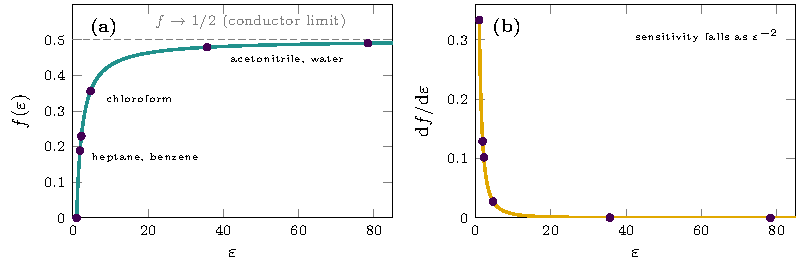
\includegraphics[width=\textwidth]{fig1_compresion.pdf}
  \caption{(a) The Kirkwood--Onsager function for the six media used here. The five
    solvents span only $0.19 \leq f \leq 0.49$ of the available range, and the two
    most polar are nearly coincident. (b) Its derivative: the sensitivity of the
    reaction field to $\varepsilon$ falls as $\varepsilon^{-2}$, so beyond
    $\varepsilon \approx 20$ the dielectric constant has almost stopped carrying
    information.}
  \label{fig:compresion}
\end{figure}

\subsection{Hypothesis}

The hypothesis tested here is that the apparent saturation of solvent effects with
$\varepsilon$ is an artefact of the chosen variable. Specifically:

\begin{enumerate}[(i)]
  \item Every quantity computed --- barrier, reaction free energy, TS bond
    distances, charge on chlorine, dipole moment --- should be a nonlinear,
    saturating function of $\varepsilon$ and a \emph{linear} function of
    $f(\varepsilon)$.
  \item The resulting straight line should have predictive value: it should give
    the barrier in a solvent that was not used to construct it, from its dielectric
    constant alone.
  \item Because a continuum model contains no solvent variable other than
    $\varepsilon$, the several correlations requested by the exercise should turn
    out to be a single correlation seen from different angles.
\end{enumerate}

\Cref{eq:onsager} is used here to identify the variable, not to compute anything:
all numbers come from the full polarizable continuum model with a molecule-shaped
cavity, not from a dipole in a sphere.

\section{Methods}

\subsection{Level of theory}

All calculations were performed with Gaussian~09~\cite{gaussian09} at the
HF/6-31+G* level, the level prescribed by the exercise. The diffuse functions
denoted by the $+$ are not optional here: the product chloride is an anion whose
density extends well beyond the valence region, and the TS carries a substantial
charge separation. The polarisation functions on heavy atoms ($*$) are needed to
describe the deformation of the carbon environment through the Walden inversion.

Hartree--Fock neglects electron correlation. This is a known and accepted
limitation of the exercise, and its probable effect on the results is discussed in
\cref{sec:limits}.

\subsection{Choice of continuum model: PCM rather than SMD}

Solvation was described with the polarizable continuum model~\cite{Tomasi2005}, in
the integral-equation formalism used by default in Gaussian~09. The cavity is built
from interlocking atom-centred spheres with radii scaled from van der Waals values;
the solute polarises the surrounding dielectric; the polarisation is represented by
apparent charges on the cavity surface; those charges generate the reaction field;
and the cycle is iterated to self-consistency with the SCF.

SMD~\cite{Marenich2009} was available and was deliberately not used. SMD computes
the same bulk-electrostatic term and adds to it a second contribution --- cavitation,
dispersion and solvent structure --- obtained as the solvent-accessible surface area
multiplied by atomic surface tensions parametrised from solvent descriptors other
than $\varepsilon$: refractive index, Abraham hydrogen-bond acidity and basicity,
macroscopic surface tension, aromaticity and halogenicity.

For predicting an experimental solvation free energy, SMD is in general the more
accurate of the two, precisely because those empirical terms absorb part of what
specific solute--solvent interactions do. For the question asked here it is the
wrong tool. The hypothesis under test is that a \emph{single} electrostatic
variable governs the solvent dependence; a model that contains several other
solvent variables by construction cannot test it. Using the less accurate model is
what makes the hypothesis falsifiable: with PCM, the only property of the solvent
that enters the calculation is $\varepsilon$, so if the correlations fail, they fail
for a reason.

\subsection{Media}

Five solvents were used --- heptane, benzene, chloroform, acetonitrile and water ---
together with the gas phase as the $\varepsilon = 1$ limit. The gas phase is not
decorative: it fixes $f(\varepsilon) = 0$ exactly, which anchors the origin of the
abscissa. Without it the five solvents span only $0.19 \leq f \leq 0.49$, and a
regression over that interval has a poorly determined intercept.

The dielectric constants used throughout are those applied internally by the
program (1.9113, 2.2706, 4.7113, 35.688 and 78.3553 respectively), read from the
output rather than taken from the handout, whose nominal values differ in the second
decimal. Since the entire analysis is a regression against a function of
$\varepsilon$, using values the calculation did not use would displace every point.

\subsection{Species, chaining and convergence strategy}

Six species were optimized and characterised by harmonic frequency calculations in
each of the six media: the reactant complex \ce{H3N\bond{...}CH3Cl}, the TS, the
separated reactants \ce{NH3} and \ce{CH3Cl}, and the products \ce{CH3NH3+} and
\ce{Cl-}. This amounts to 33 converged jobs. Every minimum gave only real
frequencies and every TS exactly one imaginary frequency, whose normal mode is the
\ce{S_{N}2} itself.

The six media were chained in a single input file per species with
\texttt{--Link1--}, each job reading the converged geometry of the previous one from
the checkpoint file. The purpose is convergence, not convenience: a TS search is
sensitive to its starting geometry, and stepping through the media in order of
$\varepsilon$ means each search begins from a structure optimized under a reaction
field only slightly different from its own.

The direction of each chain was chosen by a simple principle: \emph{start where the
starting geometry is most reliable and end where convergence is least certain}. The
reference geometries given in the handout correspond to a highly polar medium, so
the TS series was run from water downwards to the gas phase, the gas-phase TS being
the one most displaced from that reference. The reactant complex, by contrast, was
expected to be most fragile in polar media, so its series was run upwards from the
gas phase. Both expectations proved correct (\cref{sec:complex,app:failures}).

\subsection{Reference state for the barrier}

The exercise refers the barrier to the reactant complex. That reference turned out
not to exist above $\varepsilon \approx 2.3$ (\cref{sec:complex}), so barriers here
are referred to the separated reactants,
%
\begin{equation}
  \Delta G^{\ddagger} = G(\mathrm{TS}) - G(\ce{NH3}) - G(\ce{CH3Cl}).
\end{equation}
%
Besides being the only reference available in all six media, this is also the
physically appropriate one for comparison with experiment, since Menshutkin
kinetics are second order.

\subsection{Atomic charges}
\label{sec:charges}

Atomic charge is not a quantum-mechanical observable. There is no operator whose
expectation value is "the charge on chlorine"; the electron density is continuous,
and any division of it among atoms is a convention. Different conventions give
different numbers, and the choice has to be justified.

The Mulliken scheme~\cite{Mulliken1955} partitions the density according to the
basis functions it occupies: the population of each function is assigned to the atom
on which that function is centred, and overlap populations between functions on
different atoms are divided equally. Two things follow. The equal division is
arbitrary and ignores electronegativity. More seriously for the present basis, the
assignment depends on where a function is \emph{centred}, not on where the density
it carries actually is; diffuse functions extend far beyond their own centre, so
with a $+$ basis the assignment loses its meaning, and Mulliken populations are
well known not to converge as the basis set is improved.

ChelpG~\cite{Breneman1990} does not partition anything. It computes the molecular
electrostatic potential from the converged wavefunction at several thousand grid
points lying outside the van der Waals surface, and then finds by least squares the
set of atom-centred point charges that best reproduces that potential subject to the
total charge. The charges are defined by what they do rather than by how the density
is divided. Their known weakness --- that buried atoms are poorly determined, because
their charge barely affects the external potential --- does not apply to a chlorine
atom at the periphery of the molecule.

Beyond numerical stability, ChelpG is the choice consistent with the problem. A
continuum model generates its reaction field from the electrostatic potential of the
solute; defining the charges by a fit to that same potential makes the quantity
reported and the quantity driving the physics the same object. Both schemes are
compared in \cref{sec:charge-results}.

\subsection{Rate constants and data extraction}

Relative rate constants follow from transition state theory. For two media at the
same temperature the pre-exponential factors cancel, so
%
\begin{equation}
  \frac{k(\text{solvent 2})}{k(\text{solvent 1})}
  = \exp\!\left(-\frac{\Delta\Delta G^{\ddagger}}{RT}\right),
  \label{eq:tst}
\end{equation}
%
with $RT = \SI{0.592}{\kilo\calorie\per\mole}$ at \SI{298.15}{\kelvin}. The same
relation read backwards converts published relative rates into barrier differences,
which is how the comparison with experiment in \cref{sec:exp} is made.

Energies, free energies, optimized internal coordinates, ChelpG and Mulliken charges
and dipole moments were extracted from the 33 output files with an \texttt{awk}
script reproduced in \cref{app:script}, and analysed with a Python script. Both are
in the repository.

\section{Results and discussion}

\subsection{The effect does not saturate; the axis does}

\Cref{tab:data} collects the results. Correlated against $\varepsilon$, as the
exercise requests, not one of the six quantities is linear: the coefficients of
determination lie between 0.45 and 0.58. Correlated against $f(\varepsilon)$, every
one of them is a straight line, with $R^{2}$ between 0.977 and 0.9998. The points
are the same, the calculations are the same, and only the abscissa changes
(\cref{fig:main}a,b).

\begin{table}[H]
  \centering
  \caption{Transition state geometry, ChelpG charge on chlorine, dipole moment,
    imaginary frequency, activation barrier (from the separated reactants) and
    reaction free energy in the six media. The last two rows give the coefficient of
    determination of a linear fit of each column against $\varepsilon$ and against
    $f(\varepsilon)$.}
  \label{tab:data}
  \small
  \begin{tabular}{l S[table-format=2.4] S[table-format=1.3]
                    S[table-format=1.3] S[table-format=1.3]
                    S[table-format=-1.3] S[table-format=2.2]
                    S[table-format=-3.1] S[table-format=2.2] S[table-format=-3.2]}
    \toprule
    Medium & {$\varepsilon$} & {$f(\varepsilon)$} &
    {$d$(N--C)} & {$d$(C--Cl)} & {$q$(Cl)} & {$\mu$} & {$\nu^{\ddagger}$} &
    {$\Delta G^{\ddagger}$} & {$\Delta G_\mathrm{r}$} \\
    & & & {\si{\angstrom}} & {\si{\angstrom}} & {$e$} & {D} & {cm$^{-1}$} &
    \multicolumn{2}{c}{kcal/mol} \\
    \midrule
    Gas          &  1.0000 & 0.000 & 1.899 & 2.474 & -0.790 & 13.51 & -559.1 & 47.67 &  114.09 \\
    Heptane      &  1.9113 & 0.189 & 2.035 & 2.396 & -0.774 & 12.89 & -574.0 & 37.78 &   51.43 \\
    Benzene      &  2.2706 & 0.229 & 2.061 & 2.381 & -0.771 & 12.77 & -572.2 & 36.11 &   40.59 \\
    Chloroform   &  4.7113 & 0.356 & 2.136 & 2.335 & -0.761 & 12.37 & -563.8 & 31.68 &   10.85 \\
    Acetonitrile & 35.6880 & 0.479 & 2.203 & 2.292 & -0.749 & 12.00 & -554.5 & 28.24 &  -12.97 \\
    Water        & 78.3553 & 0.490 & 2.209 & 2.289 & -0.748 & 11.96 & -553.6 & 27.97 &  -14.93 \\
    \midrule
    $R^{2}$ vs.\ $\varepsilon$    & {--} & {--} & 0.510 & 0.527 & 0.576 & 0.549 & {--} & 0.447 & 0.464 \\
    $R^{2}$ vs.\ $f(\varepsilon)$ & {--} & {--} & 0.995 & 0.998 & 0.999 & 1.000 & {--} & 0.977 & 0.983 \\
    \bottomrule
  \end{tabular}
\end{table}

\begin{figure}[H]
  \centering
  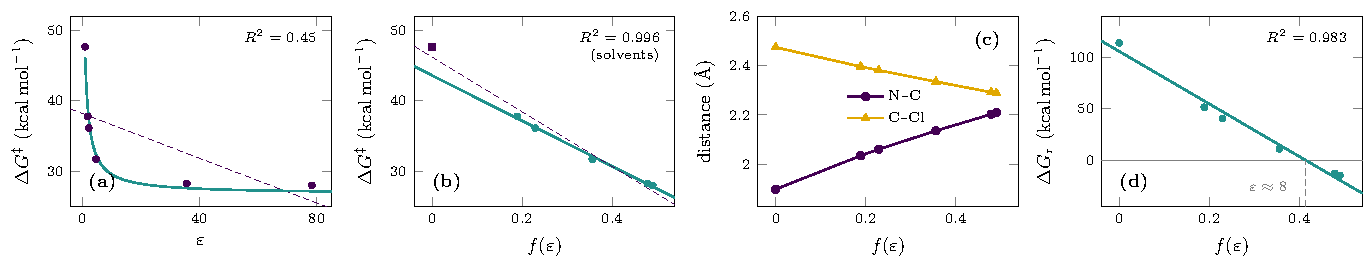
\includegraphics[width=\textwidth]{fig2_principal.pdf}
  \caption{(a) Activation barrier against $\varepsilon$. The dashed line is the
    linear fit the exercise invites ($R^{2} = 0.45$); the solid line is the model of
    panel (b) mapped back onto this axis, showing that the data are not scattered but
    simply not linear in $\varepsilon$. (b) The same barriers against
    $f(\varepsilon)$: solid, the fit to the five solvents; dashed, the fit including
    the gas phase. (c) TS bond distances and (d) reaction free energy against
    $f(\varepsilon)$; the vertical line in (d) marks where the reaction becomes
    exergonic.}
  \label{fig:main}
\end{figure}

It is worth being explicit about what this does and does not show. It does not show
that $f(\varepsilon)$ is a better fitting function than $\varepsilon$ in some
statistical sense; with six points and two parameters that would mean little. It
shows that the \emph{same} six points give $R^{2} \approx 0.5$ on one axis and
$R^{2} \approx 0.99$ on another, and that the second axis is the one the theory of
the method says should appear. The statistics are a consequence of the physics, not
a substitute for it.

\subsection{A predictive model and its range of validity}

The five solvents define
%
\begin{equation}
  \Delta G^{\ddagger} = -32.2\,f(\varepsilon) + 43.6
  \quad\text{kcal/mol},\qquad R^{2} = 0.996 .
  \label{eq:fit}
\end{equation}
%
This is more than a description. It predicts the barrier in any solvent from its
dielectric constant alone, without a further calculation.
\Cref{tab:loo} tests it by leave-one-out cross-validation: each medium is predicted
from a fit to the other five.

\begin{table}[H]
  \centering
  \caption{Leave-one-out validation of \cref{eq:fit}. Each row is predicted from a
    straight line fitted to the other five media.}
  \label{tab:loo}
  \small
  \begin{tabular}{l S[table-format=1.4] S[table-format=2.2] S[table-format=2.2] S[table-format=-1.2]}
    \toprule
    Medium & {$f(\varepsilon)$} & {predicted} & {calculated} & {error} \\
    & & \multicolumn{3}{c}{kcal/mol} \\
    \midrule
    Gas          & 0.0000 & 43.59 & 47.67 & -4.08 \\
    Heptane      & 0.1890 & 39.17 & 37.78 &  1.39 \\
    Benzene      & 0.2293 & 37.57 & 36.11 &  1.46 \\
    Chloroform   & 0.3561 & 32.53 & 31.68 &  0.85 \\
    Acetonitrile & 0.4793 & 27.20 & 28.24 & -1.04 \\
    Water        & 0.4905 & 26.62 & 27.97 & -1.35 \\
    \bottomrule
  \end{tabular}
\end{table}

The five solvents are reproduced to within \SI{1.5}{\kilo\calorie\per\mole}. The gas
phase is not: it is predicted \SI{4.1}{\kilo\calorie\per\mole} too low, and
including it in the fit degrades $R^{2}$ from 0.996 to 0.977 and changes the slope
from $-32.2$ to $-38.9$.

The deviation is not noise and it has a specific cause. \Cref{eq:onsager} is linear
in $f(\varepsilon)$ \emph{at constant $\mu$}; the dipole moment of the TS is not
constant, falling from \SI{13.51}{\debye} in the gas phase to \SI{11.96}{\debye} in
water (\cref{tab:data}). The gas phase is the point whose dipole departs furthest
from the rest, and it deviates furthest from the line. The practical consequence is
that \cref{eq:fit} should be used to interpolate between solvents and not to
extrapolate to vacuum --- which is also the regime in which a continuum model has
nothing to describe.

\subsection{The reactant complex is screened out of existence}
\label{sec:complex}

The exercise assumes a reactant complex \ce{H3N\bond{...}CH3Cl} from which the
barrier is measured. In the gas phase it exists, but barely: the complexation
energy is \SI{-1.56}{\kilo\calorie\per\mole}, consistent with a dipole--dipole
interaction between two small neutral molecules. A dielectric medium screens such an
interaction, and the screening is visible immediately (\cref{tab:complex}).

\begin{table}[H]
  \centering
  \caption{Complexation energy and free energy of \ce{H3N\bond{...}CH3Cl} in the
    media where the complex is a minimum. Beyond benzene no minimum was located.}
  \label{tab:complex}
  \small
  \begin{tabular}{l S[table-format=1.4] S[table-format=-1.2] S[table-format=1.2]}
    \toprule
    Medium & {$f(\varepsilon)$} & {$\Delta E_\mathrm{cplx}$} & {$\Delta G_\mathrm{cplx}$} \\
    & & \multicolumn{2}{c}{kcal/mol} \\
    \midrule
    Gas     & 0.0000 & -1.56 & 3.24 \\
    Heptane & 0.1890 & -0.88 & 3.99 \\
    Benzene & 0.2293 & -0.73 & 4.21 \\
    \bottomrule
  \end{tabular}
\end{table}

In chloroform and above, the optimization does not converge, and the reason is
instructive rather than technical. Over the last hundred optimization cycles the
energy varies by less than \SI{0.001}{\kilo\calorie\per\mole} while the N--C
distance drifts past \SI{7}{\angstrom}: the surface has become flat, and there is no
minimum to converge to. The failure is a measurement of the screening, not an
artefact of it. The same phenomenon was observed in session~4 for the ion--dipole
complexes of \ce{F- + CH3Cl}, which disappear in water; there the interaction was
ion--dipole and survived to $\varepsilon = 78$, here it is dipole--dipole and does
not survive $\varepsilon = 4.7$.

A second observation makes the choice of reference unavoidable. Even where the
complex exists, its complexation \emph{free} energy is positive:
\SIrange{3.2}{4.2}{\kilo\calorie\per\mole}. Associating two molecules into one costs
translational and rotational entropy, about
\SI{6}{\kilo\calorie\per\mole} at room temperature, which exceeds a binding energy of
one or two. The complex is therefore above the separated reactants in free energy
even when it is below them in electronic energy, and the separated reactants are the
better reference on thermodynamic as well as practical grounds.

\subsection{Geometry, charge and dipole: an earlier and less polarised TS}
\label{sec:charge-results}

Two of the computed quantities behave opposite to naive expectation. As the medium
becomes more polar, the charge on chlorine becomes \emph{less} negative, from
$-0.790$ to $-0.748\,e$, and the dipole moment of the TS \emph{falls}, from
\SIrange{13.51}{11.96}{\debye} (\cref{fig:cargas}). The TS is less polarised in
water than in vacuum.

\begin{figure}[H]
  \centering
  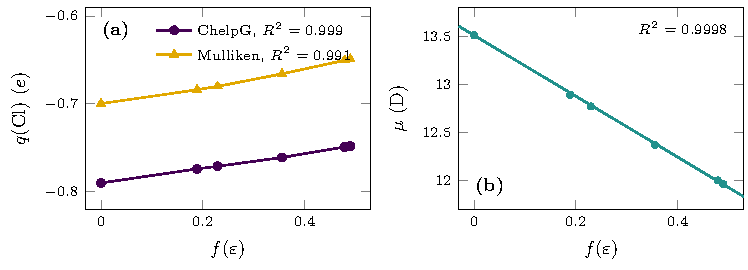
\includegraphics[width=\textwidth]{fig3_cargas.pdf}
  \caption{(a) Charge on chlorine against $f(\varepsilon)$ computed with ChelpG and
    with Mulliken population analysis. The absolute values differ by about
    $0.09\,e$, which is the arbitrariness of the convention, but the trend and the
    linearity against $f(\varepsilon)$ are the same. (b) Dipole moment of the TS,
    the most nearly linear of all the quantities computed.}
  \label{fig:cargas}
\end{figure}

A reaction field polarises a solute, so the direct effect of increasing
$\varepsilon$ should be to increase $\mu$ and the charge separation. Something
larger is working in the opposite direction, and \cref{tab:data} identifies it: the
geometry. The N--C distance lengthens from \SIrange{1.899}{2.209}{\angstrom} while
the C--Cl distance shortens from \SIrange{2.474}{2.289}{\angstrom}. The TS moves
\emph{earlier} along the reaction coordinate as the solvent becomes more polar, and
an earlier TS has transferred less charge. The geometric displacement overrides the
direct polarisation.

That the dipole moment is the quantity that correlates best of all
($R^{2} = 0.9998$) is worth noting, because it is also the quantity that appears
explicitly in \cref{eq:onsager}. The chain $f(\varepsilon) \rightarrow$ reaction
field $\rightarrow$ geometry $\rightarrow$ dipole closes on itself.

\subsection{Hammond's postulate, measured}

The reason the TS moves is thermodynamic. \Cref{fig:main}d shows the reaction free
energy: \SI{+114.09}{\kilo\calorie\per\mole} in the gas phase, where the products
are two separated ions in vacuum, falling to \SI{-14.93}{\kilo\calorie\per\mole} in
water. The solvent swings the thermodynamics of the reaction by
\SI{129}{\kilo\calorie\per\mole} and turns it from impossible to spontaneous.

Hammond's postulate then requires the TS of a strongly endergonic reaction to
resemble the products, and that of a less endergonic one to move back towards the
reactants. \Cref{fig:hammond} tests this directly rather than by inspection.

\begin{figure}[H]
  \centering
  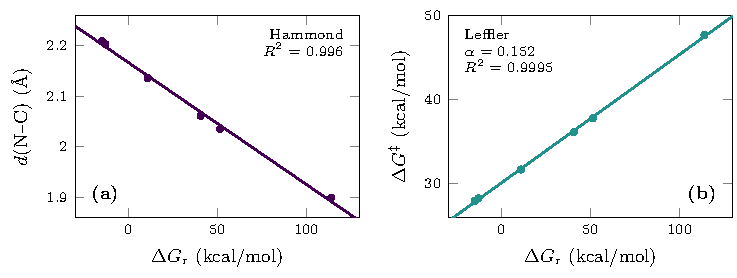
\includegraphics[width=\textwidth]{fig4_hammond.pdf}
  \caption{(a) Position of the transition state, measured by the forming N--C bond,
    against the reaction free energy: Hammond's postulate as a quantitative
    relation. (b) Barrier against reaction free energy; the slope is the Leffler
    coefficient $\alpha$.}
  \label{fig:hammond}
\end{figure}

The forming bond tracks the thermodynamics with $R^{2} = 0.996$, and the barrier
tracks it with $R^{2} = 0.9995$ and slope
%
\begin{equation}
  \alpha = \frac{\partial \Delta G^{\ddagger}}{\partial \Delta G_\mathrm{r}} = 0.152 ,
\end{equation}
%
the Leffler coefficient. A value near zero describes a reactant-like TS, one near
unity a product-like one, and $0.15$ places this TS early over the range sampled,
consistent with the geometries.

Extrapolating the fit of \cref{fig:main}d, the reaction becomes exergonic at
$f(\varepsilon) = 0.414$, that is $\varepsilon \approx 8$. This is a concrete and
testable prediction, and it agrees with synthetic practice: Menshutkin alkylations
are run in acetonitrile, DMSO or nitrobenzene, and not in hexane or toluene.

\subsection{One variable, five correlations}

The correlations above are not independent, and saying so is part of reporting them
honestly.

In a continuum model the only property of the solvent that enters the calculation is
$\varepsilon$, and it enters only through $f(\varepsilon)$. Every converged property
of the solute --- its geometry, its charge distribution, its energy --- is therefore a
function of that single variable. If each of them is linear in $f(\varepsilon)$ over
the range sampled, then each is necessarily linear in each of the others. The
Hammond relation of \cref{fig:hammond}a and the Leffler relation of
\cref{fig:hammond}b follow from that common dependence; they do not constitute
independent evidence for it.

What does carry physical content is not the existence of the correlations but their
slopes. That $\alpha = 0.15$ rather than $0.85$ is a statement about this transition
state that no amount of common dependence could have produced; that the barrier
falls by \SI{32}{\kilo\calorie\per\mole} across the full range of
$f(\varepsilon)$ is a statement about this reaction.

The conclusion is also independent of the charge partition scheme, which is the
obvious objection to any discussion built on atomic charges. Mulliken populations
differ from ChelpG by about $0.09\,e$ in absolute value, as expected from two
different conventions, but give the same trend, the same sign and the same
qualitative contrast between the two axes: $R^{2} = 0.62$ against $\varepsilon$ and
$0.99$ against $f(\varepsilon)$ (\cref{fig:cargas}a).

\subsection{Comparison with experiment}
\label{sec:exp}

The calculation predicts that the barrier falls by
\SI{9.5}{\kilo\calorie\per\mole} between heptane and acetonitrile. Published
Menshutkin rate data, converted to barrier differences with \cref{eq:tst}, give
about \SI{5.6}{\kilo\calorie\per\mole} over the same range of polarity
(\cref{tab:exp}).

\begin{table}[H]
  \centering
  \caption{Experimental relative rates for Menshutkin reactions~\cite{Reichardt2011}
    converted into barrier differences with \cref{eq:tst} at \SI{298}{\kelvin}.}
  \label{tab:exp}
  \small
  \begin{tabular}{l S[table-format=2.1] S[table-format=5.0] S[table-format=1.2]}
    \toprule
    Solvent (relative to hexane) & {$\varepsilon$} & {$k_\mathrm{rel}$} &
    {$-\Delta\Delta G^{\ddagger}$ (kcal/mol)} \\
    \midrule
    Carbon tetrachloride &  2.2 &    31 & 2.03 \\
    Chlorobenzene        &  5.6 &  1200 & 4.20 \\
    Acetonitrile         & 37.5 & 12000 & 5.56 \\
    Dimethyl sulfoxide   & 46.7 & 50000 & 6.41 \\
    \bottomrule
  \end{tabular}
\end{table}

The direction is right and the order of magnitude is right; the effect is
overestimated by nearly a factor of two. Three contributions are expected, and it is
worth separating them because they are not equally fundamental.

The first is the system. The experimental data are for tertiary amines and alkyl
iodides, not for \ce{NH3} and \ce{CH3Cl}; a more nucleophilic amine and a better
leaving group give a different, and generally earlier, TS. This is a comparison of
trends between related systems, not of absolute barriers, and only the trends should
be expected to agree.

The second is the method. Hartree--Fock has no electron correlation, and there is no
reason for the correlation energy to cancel between a pair of neutral closed-shell
molecules and a strongly polarised TS. Correlation typically stabilises the more
polarisable species, which here is the TS, so a correlated method would be expected
to lower the barriers --- but not uniformly across media, so the slope would change
too.

The third is the solvent model, and it is the most interesting. A continuum contains
no solvent molecules and therefore no specific hydrogen bonds. In protic media the
developing chloride is stabilised by hydrogen bonding that PCM represents only as
bulk polarisation of a dielectric. The effect of adding explicit solvent molecules
would not be a uniform shift: it would act mainly at the polar end of the series,
where it would stabilise the TS further.

\subsection{What this analysis cannot say}
\label{sec:limits}

Three limitations should be stated plainly.

The analysis is internal to the continuum approximation. It establishes that, within
a model whose only solvent parameter is $\varepsilon$, the correct variable is
$f(\varepsilon)$. It does not establish that real solvent effects are linear in
$f(\varepsilon)$, and for protic solvents they are known not to be.

The cavity is not a sphere. \Cref{eq:onsager} was derived for a point dipole in a
spherical cavity, whereas PCM uses a molecule-shaped cavity and the full charge
distribution. That the numerical model reproduces the functional form of the
analytical one is an empirical finding of this work, not a theorem; it holds because
the boundary conditions are the same and the solute is reasonably compact.

Six points is not many. The conclusion rests on the contrast between $R^{2}
\approx 0.5$ and $R^{2} \approx 0.99$ on the same data, which is large enough to be
safe, but the slopes of the individual fits carry a correspondingly wide uncertainty
that has not been propagated.

\section{Conclusions}

\begin{enumerate}
  \item Correlating against $\varepsilon$, as the exercise requests, gives no linear
    relationship for any of the six quantities computed
    ($0.45 \leq R^{2} \leq 0.58$). Correlating the same data against
    $f(\varepsilon) = (\varepsilon-1)/(2\varepsilon+1)$, the function in which
    $\varepsilon$ actually appears in the theory of the method, gives a straight
    line for all of them ($0.977 \leq R^{2} \leq 0.9998$). The apparent saturation
    of solvent effects is a property of the axis, not of the chemistry.

  \item The resulting line, $\Delta G^{\ddagger} = -32.2\,f(\varepsilon) + 43.6$
    kcal/mol, predicts the barrier in a solvent omitted from the fit to within
    \SI{1.5}{\kilo\calorie\per\mole}. It should not be extrapolated to the gas
    phase, where the assumption of constant $\mu$ behind the linearity fails.

  \item Since $f(\varepsilon)$ is the only solvent variable a continuum model
    contains, the several correlations requested by the exercise are in fact one
    correlation, and only their slopes carry independent information.

  \item Those slopes are chemically sensible. The solvent swings the reaction free
    energy by \SI{129}{\kilo\calorie\per\mole}, turning the reaction exergonic above
    $\varepsilon \approx 8$, and displaces the transition state earlier along the
    reaction coordinate (Leffler $\alpha = 0.15$), which leaves it \emph{less}
    polarised in water than in vacuum --- the opposite of what direct polarisation of
    the solute alone would give.

  \item The reactant complex assumed by the exercise is screened out of existence
    above $\varepsilon \approx 2.3$, and is above the separated reactants in free
    energy even where it exists. Barriers must be referred to the separated
    reactants, which is also what the second-order experimental kinetics require.

  \item Against experiment the model reproduces the direction and the order of
    magnitude of the solvent effect (\SI{9.5}{} against
    \SI{5.6}{\kilo\calorie\per\mole} between heptane and acetonitrile) but
    overestimates it, as expected from a method without electron correlation and a
    continuum model without hydrogen bonds.
\end{enumerate}

\appendix

\section{Calculations that failed, and what they showed}
\label{app:failures}

Two of the 35 jobs attempted did not converge. Both are reported because in one case
the failure was the result.

\textbf{The reactant complex beyond benzene.} The chained optimization terminated in
link 9999 after exhausting 100 cycles. Inspection of the trajectory showed the
energy constant to within \SI{0.001}{\kilo\calorie\per\mole} over the last hundred
steps while $d$(N--C) drifted past \SI{7}{\angstrom}. No tighter convergence
criterion or larger cycle limit would have helped: there was no stationary point.
This is reported in \cref{sec:complex} as a result.

\textbf{The methylammonium cation beyond heptane.} The same link-9999 termination
after 38 cycles, but here the cause was numerical. The job had been set up with a
plain \texttt{opt} keyword and an estimated Hessian, which is adequate in the gas
phase but not on the flatter surface produced by a reaction field. Repeating the
four remaining media with \texttt{opt=(calcfc,maxcycles=200)}, so that the Hessian
is computed rather than guessed, converged all of them without further difficulty.

The contrast between the two is the practical lesson: an optimization that fails
because the surface is flat and one that fails because the optimizer is badly
initialised produce the same error message, and are distinguished by looking at the
energy along the trajectory rather than at the final geometry.

\section{Extraction script}
\label{app:script}

The following \texttt{awk} program reads any number of Gaussian output files and
emits one record per converged job. It is reproduced here because the choice of
patterns encodes several non-obvious features of the output format.

\begin{verbatim}
/^ Solvent  / {
    sol = $3; sub(/,$/, "", sol)
    split($0, p, "Eps="); eps = p[2] + 0
}
/^ SCF Done:/            { e = $5 }
$1 == "!" && $2 == "r1"  { rnc  = $3 }
$1 == "!" && $2 == "r5"  { rccl = $3 }
/^ ESP charges:$/        { inesp = 1; next }
inesp && $2 == "Cl"      { q = $3; inesp = 0 }
/Dipole moment \(field-independent/ { getline; mu = $NF }
/^ Frequencies --/       { if (nu == "") nu = $3 }
/Sum of electronic and thermal Free Energies=/ {
    print ...; sol = ""; eps = 0; rnc = ""; rccl = ""; q = ""; nu = ""
}
\end{verbatim}

Three points are worth noting. The solvent and its dielectric constant are read from
the \texttt{Solvent} banner rather than from the route line, so that the value used
is the one the program actually applied. The pattern for the charges is anchored at
both ends, \verb|/^ ESP charges:$/|, because Gaussian prints three blocks whose
headers all contain that string and only one of which is wanted. And the record is
emitted on the thermochemistry line rather than on \texttt{Normal termination},
because a job that failed never reaches the former --- which is why the failed jobs
simply do not appear in the output rather than appearing with corrupt values.

{\small
\bibliographystyle{unsrt}
\bibliography{bibliografia}
}

\end{document}
